
\subsection{Application on MNIST}
For k = 1024 and $\mu = 5$:

\begin{figure}[h]
 \centering
 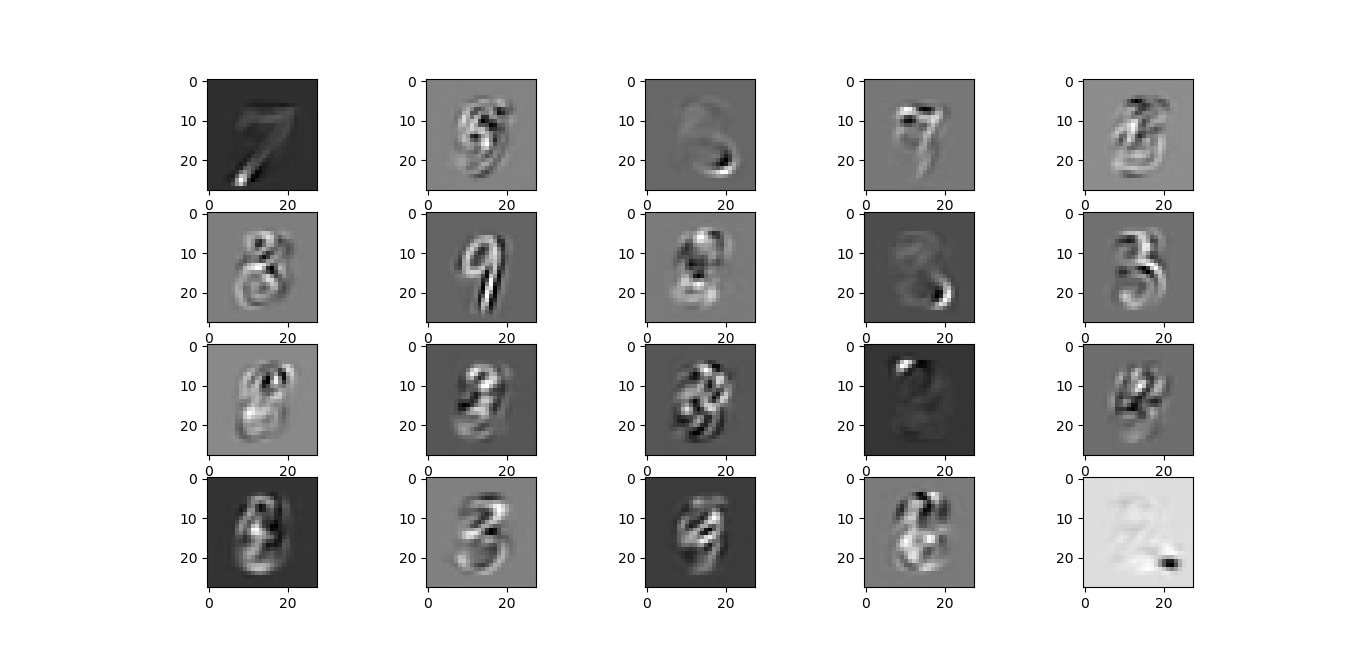
\includegraphics[scale=0.5]{../Results/LC-KSVD_X_ALL_K_1024/D.png}
 % D.png: 1366x660 px, 100dpi, 34.70x16.76 cm, bb=0 0 984 475
 \caption{Examples of D's atoms}
\end{figure}

\begin{figure}[h]
 \centering
 \includegraphics[scale=0.5]{../Results/LC-KSVD_X_ALL_K_1024/repartition_h.png}
 % répartition_h.png: 681x651 px, 100dpi, 17.30x16.54 cm, bb=0 0 490 469
 \caption{Sparse coefficients repartition}
\end{figure}
\begin{figure}[h]
 \centering
 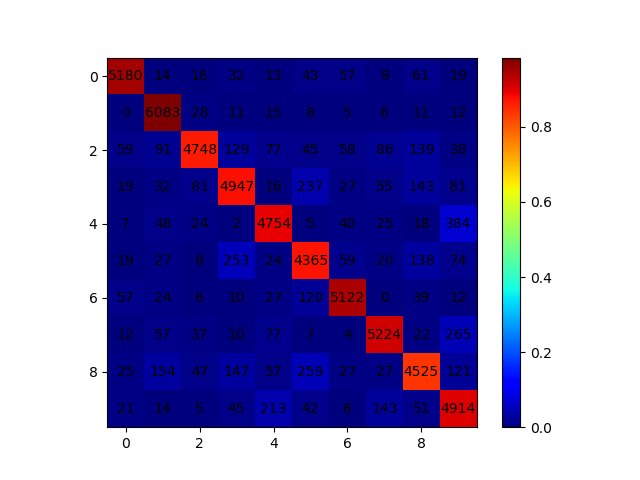
\includegraphics[scale=0.72]{../Results/LC-KSVD_X_ALL_K_1024/confusion_matrix_train.png}
 % confusion_matrix_train.png: 640x480 px, 100dpi, 16.26x12.19 cm, bb=0 0 461 346
 \caption{Kmeans classification on A$\alpha$ from the trainning dataset}
\end{figure}


 \begin{figure}[h]
 \begin{subfigure}{.5\textwidth}
 \centering
 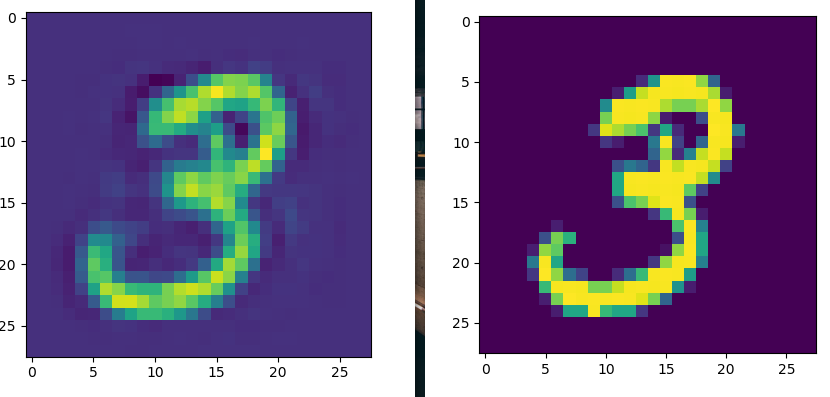
\includegraphics[scale=0.29]{../Results/LC-KSVD_X_ALL_K_1024/3_recons.png}
  \caption{Reconstructed 3 vs Original 3}
 % module-capteur-laser.jpg: 600x600 px, 72dpi, 21.17x21.17 cm, bb=0 0 600 600
 \end{subfigure}%
  \begin{subfigure}{.3\textwidth}
 \centering
 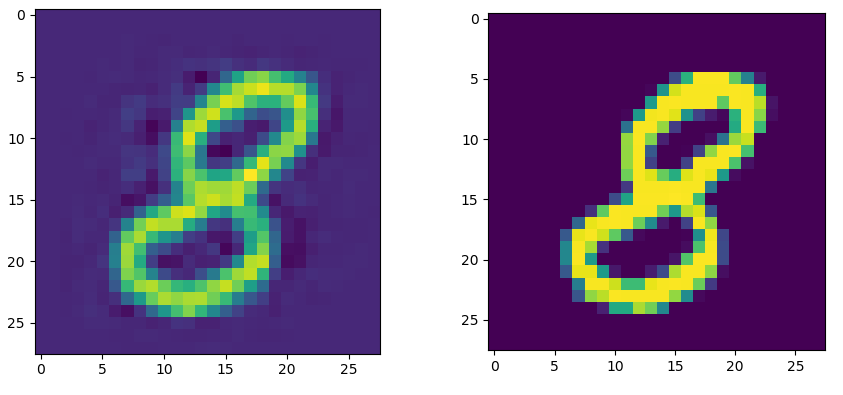
\includegraphics[scale=0.29]{../Results/LC-KSVD_X_ALL_K_1024/8_recons.png}
 % module-capteur-laser.jpg: 600x600 px, 72dpi, 21.17x21.17 cm, bb=0 0 600 600
  \caption{Reconstructed 8 vs Original }

 \end{subfigure}%
\end{figure}

\begin{figure}[h!]
 \centering
 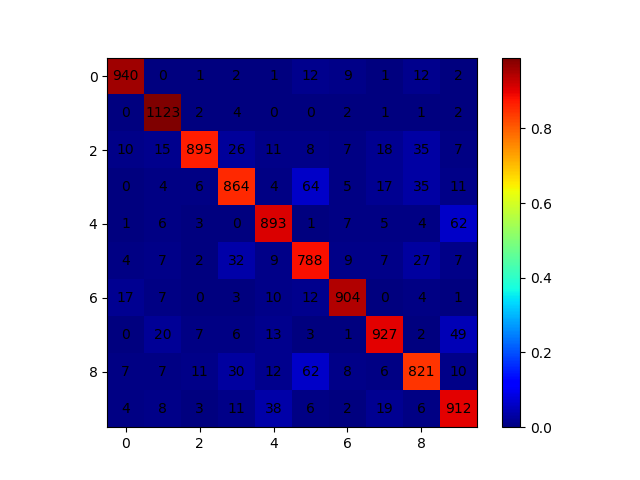
\includegraphics[scale=0.72]{../Results/LC-KSVD_X_ALL_K_1024/confusion_matrix_test.png}
 % confusion_matrix_test.png: 640x480 px, 100dpi, 16.26x12.19 cm, bb=0 0 461 346
 \caption{Kmeans classification on A $\alpha$ from the test dataset w}
\end{figure}
